\chapter{Jet Energy Scale}
\label{JES}

Recalling from Sec.~\ref{jets} that jets evolve through many different stages throughout their life (see Fig.~\ref{JetLevelsFig}) it becomes clear that to reasonably compare experimental results to theoretical results one must decide on a scale to make the comparison at.  
This is usually done by bringing all results to the `particle jet' scale, making the results detector independent easing cross experiment comparisons.  
This is accomplished by carefully studying the relationship between the particle scale jet energy and the detector scale jet energy, known as the \gls{JES}.   
A successful \gls{JES} accounts for pileup, escaped/invisible energy, algorithm effects, etc.  


\begin{figure}[!ht]
  \begin{center}
    \scalebox{0.40}{
      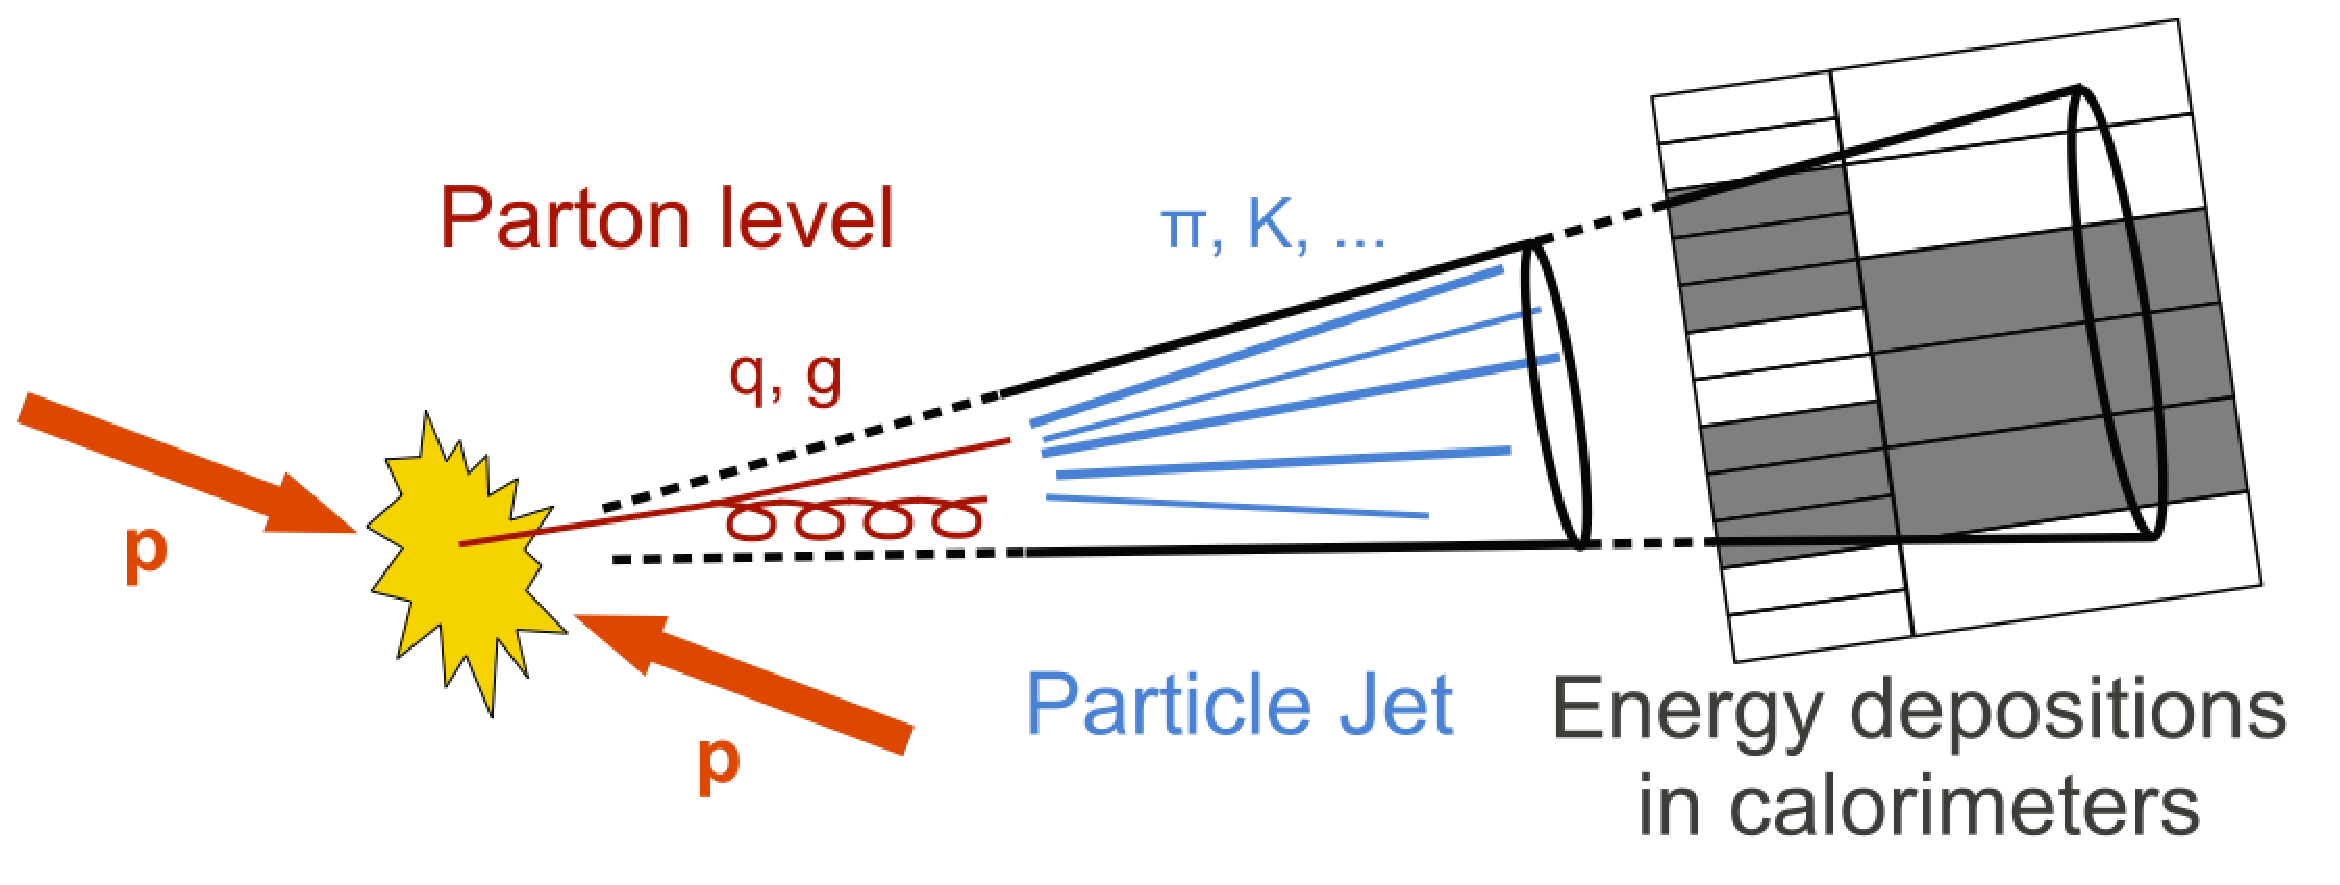
\includegraphics{plots/Chap4/Sketch_PartonParticleCaloJet.eps}
    }
  \end{center}
  \caption[Jet showering evolution.]
      {\small A cartoon outlining the progression from parton level to a calorimeter jet.}
  \label{JetLevelsFig}
\end{figure}

\section{Jet Energy Scale in ATLAS}
\label{ATLASJES}

Calibrating jets withing ATLAS is a multistaged process.  
During the initial jet reconstruction the jet is set to originate from point (0,0,0) in the ATLAS coordinate system, so the first step is to adjust the jet to originate from the reconstructed vertex.  
Next in order to compensate for energy coming from previous collisions and secondary interactions energy is subtracted from the jet, first using the average energy density observe in that given event along with the active area of the jet (calculated using ghost particles~\cite{Soyez:2012hv}) followed by a smaller residual correction.  
With pileup now removed a Monte Carlo based calibration, which completely corrects for the average response as a function of energy and pseudorapidity of jet within that sample, is applied.  

To improve the energy resolution and reduce the flavour dependence of the jets at this stage a series of smaller Monte Carlo calibration are applied.  
These calibrations ideally flatten the dependence of the response on the amount of energy in the first layer of the hadronic calorimeter, the energy in the last layer of the EM calorimeter, the number of charged tracks within the jet, the width of the distribution of those tracks within the jet, and the number of track segments in the muon spectrometer behind the jet.  
These calibrations are collectively known as the \gls{GSC}.  

\begin{figure}[!ht]
  \begin{center}
    \scalebox{0.40}{
      \includegraphics{plots/Chap4/CalibSequence.ps}
    }
  \end{center}
  \caption[Jet showering evolution.]
      {\small A cartoon outlining the progression from parton level to a calorimeter jet.}
  \label{JetCalibSequenceFig}
\end{figure}


The final step involves applying final corrections to account for the observed differences in response between the data which has been collected and the Monte Carlo.  
The response is measured using a series of \textit{in-situ} techniques in both data and Monte Carlo, and the ratio is applied as a final correction to data only.  
In general these \textit{in-situ} techniques make use of a system of physics objects which have been produced back-to-back in $\phi$.  
One object is labeled as the reference object and the response of the second object is measured relative to the reference object.  
These studies can be performed in dijet events where the jets land in different $\eta$ regions (so called eta intercalibration), $\gamma$/Z+jet events where the jet response is measured relative to the boson, and multi jet events where one high energy jet is measured relative to several lower energy jets.  

This study will be using both Z and $\gamma$+jet events to study the jet energy scale in ATLAS.  
Only events where the Z decays into either an electron/positron pair or a muon/anti-muon pair will be considered.  
When it comes to measuring the JES these two types of events are similar and complementary.  
Both offer well measured objects which are ideally produced back-to-back in $\phi$ with a single jet, with a significant difference being that the cross section for $\gamma$+jet is several orders of magnitude larger.   
This larger cross section allows for a larger number of high energy $\gamma$+jet events, stretching out the range which can be calibrated.  
Unfortunately this larger cross section also forces lower energy photon triggers to be prescaled to much lower rates.  
This prescaling at low energy, along with a large number of low energy dijet events being misidentified as $\gamma$+jet events makes Z+jet a much better choice while calibrating the low energy regime.  

\section{Jet Response}

The largest component of the JES is the absolute response, which describes how the calorimeter response to both hadronic and electromagnetic energy deposits within the jet.  
Even for a single incoming hadron there will be some fraction of energy deposited in the calorimeter via EM interactions.  
This is in part because hadrons do have electric charge, but is largely due to hadrons decaying into particles which decay electromagnetically ($\pi^0\rightarrow\gamma\gamma$).  
If we use this division in energy deposit type to write a single particle response, we can say

\begin{equation}
  \label{SingleParticleResponse}
  r(E)=f_{\mathrm{em}}\left(E\right)e+\left[1-f_{\mathrm{em}}\right]\left(E\right)h,
 \end{equation}

\noindent
where $e$ is the response to purely EM energy deposits, $h$ is the response to purely hadronic energy deposits, and $f_{\mathrm{em}}$ is the fraction of the total incoming energy that is deposited electromagnetically.  

This can be further explored by using a simplistic model of a particle showering within a material.  
When a hadron interacts with a nucleus several new hadrons are created, with pions being produced in the largest numbers.  
Thanks to the approximate isospin symmetry of hadronic interactions each flavour of pions is created with equal probability, so if only pions are produced in a given interaction on average 1/3 of these pions will be electromagnetically decaying neutral pions.  
With this model in mind after the first generation of hadrons is produced 1/3 of the available energy is electromagnetic energy deposited by photons resulting from the decay of neutral pions.  
If the charged pions making up the remaining 2/3 of the available energy each have enough energy to cause a subsequent shower, a further 2/9$^{\mathrm{ths}}$ of the energy will be deposited electromagnetically, and so on.  
This dependence of the fraction of EM energy on the total energy of the incident particle can be modeled using

\begin{equation}
  \label{Grooms}
  f_{\mathrm{em}}\left(E\right)=1-\left(\frac{E}{E_0}\right)^{m-1}.
\end{equation} 

\noindent 
Another function which has been used to model the EM fraction with success is 
\begin{equation}
  \label{Wigmans}
  f_{\mathrm{em}}\left(E\right)=a_0+a_1\mathrm{ln}\frac{E}{E_{\mathrm{scale}}}+a_2\left(\mathrm{ln}\frac{E}{E_{\mathrm{scale}}}\right)^2.
\end{equation}

The response of an entire jet can be modeled using
\begin{equation}
  R_{\mathrm{jet}}\left(E\right)=w_hr\left(w_hE\right)+w_ee\left(w_eE\right)
\end{equation}
along with Eq.~\ref{SingleParticleResponse} and either Eq.~\ref{Grooms} or Eq.~\ref{Wigmans}, where $w_h$ and  $w_e$ are the fraction of particles in the jet which will interact hadronically or electromagnetically, respectively.  
These quantities are solely dependent on the parton shower and hadronization processes and are independent of any subsequent showering within the detector.   

\section{$E_{\mathrm T}^{miss}$ Projection Method}
\label{METProj}

The Missing $E_{\mathrm T}$ projecting fraction method is an \textit{in-situ} technique for measuring the jet response.  
It was first developed at the CDF collaboration~\cite{abe1992dijet} to help with their $\eta$ intercalibration, and was later used by the D0 collaboration to extract an absolute jet energy scale~\cite{item/10150/186444}.  
As opposed to the $p_{\mathrm T}$ balance method, which directly compares the measured energy of the jet to the reference object, the MPF measures the response of the entire recoiling system.

The MPF does this using only the measured probe energy and the MET, removing the need to explicitly include the measured jet energy in the response measurement making it independent of the jet algorithm that was used.  
It should be noted that the response still depends on the inputs to the jet finding algorithm, and therefore a MET at the appropriate scale must be used.  
This absence of jet information in the calibration does mean that to perform a full \textit{in-situ} calibration additional algorithm/jet size related corrections do need to be derived.  
This downside can be compensated by the MPF's ability to much more resilient to initial/final state radiation, allowing for looser selection criteria and a relatively larger sample size, as well as its ability to be relatively unaffected by pileup.  

The MPF does take advantage of the balance between the reference object and the recoiling parton to obtain a measure of the true momentum in the recoil, so the derivation of the MPF response begins with 
\begin{equation}
  \label{EQ:MPFPartonLevel}
  \vec{p}_{\mathrm T}^{\mathrm{ref}}+\vec{p}_{\mathrm T}^{\mathrm{recoil}} = 0.  
\end{equation}
\noindent
where $\vec{p}_{\mathrm T}$ is the shorthand for the total momentum of a given particle/object projected into the transverse plane.   
We must also consider this balance at the calorimeter level, which in the simple case of a $2\rightarrow$2 collision can be written as
\begin{equation}
  \label{EQ:MPFCaloLevel}
  R_{\mathrm{ref}}\vec{E}_{mathrm T}^{\mathrm{ref}}+R_{\mathrm{recoil}}\vec{E}_{mathrm T}^{\mathrm{recoil}}=-\vec{E}_{mathrm T}^{\mathrm{miss}},
\end{equation}
\noindent
where we are using $R_{\mathrm{object}}$ to be the response of the calorimeter to that object, and $\vec{E}_{mathrm T}^{\mathrm{object}}$ is known as the transverse energy of the object which is defined as
\begin{equation}
  \vec{E}_{mathrm T}=\frac{E}{\mathrm{cosh}\left(\eta\right)}\hat{p}_{mathrm T}.  
\end{equation}
\noindent
In this thesis only well measured objects are used as references, so $R_{\mathrm{ref}}\simeq1$ and small differences are well known and can be propagated to $\vec{E}_{mathrm T}^{\mathrm{miss}}$.  
By projecting both sides of Eq.~\ref{EQ:MPFCaloLevel} along the directions of the reference object and using Eq.~\ref{EQ:MPFPartonLevel} to remove ${E}_{mathrm T}^{\mathrm{recoil}}$ we obtain
\begin{equation}
  E_{mathrm T}^{\mathrm{ref}}-R_{\mathrm{recoil}}E_{mathrm T}^{\mathrm{ref}}=-\vec{E}_{mathrm T}^{\mathrm{miss}}\cdot\hat{p}_{mathrm T}^{\mathrm{ref}}.
\end{equation} 

\begin{equation}
  \label{EQ:MPFSimple}
  R_{\mathrm{recoil}}=1+\frac{\vec{E}_{mathrm T}^{\mathrm{miss}}\cdot\hat{p}_{mathrm T}^{\mathrm{ref}}}{E_{mathrm T}^{\mathrm{ref}}}.
\end{equation}

This is the MPF that is used to measure the JES \textit{in-situ}.  
What exactly the MPF is doing can be made more clear by expanding out the MET.  
In this ideal case where only the reference object and the recoil exist (using Eq.~\ref{EQ:MPFCaloLevel}) we get that the MPF is just the ratio of the measured energy of the recoil to the measured energy of the reference object.  
In practice the MET will include both initial and final state radiation (ISR and FSR), the underlying event, and pileup.  
This means that the MET can be written as 
\begin{equation}
  \vec{E}_{mathrm T}^{\mathrm{miss}} = -\vec{E}_{T}^{\mathrm{ref}}-\sum_{n}\vec{E}_{mathrm T}^{n},
\end{equation}
where n runs over all energy deposits in the calorimeter that are no related to the reference object.  
Using this definition of the MET we see that the MPF can be written as 
\begin{equation}
  R_{\mathrm{recoil}}=1-\frac{E_{mathrm T}^{\mathrm{ref}}+\hat{p}_{mathrm T}^{\mathrm{ref}}\cdot\sum_{n}\vec{E}_{mathrm T}^{n}}{E_{mathrm T}^{\mathrm{ref}}}=-\frac{\sum_{n}\vec{E}_{mathrm T}^{n}\cdot\hat{p}_{mathrm T}^{\mathrm{ref}}}{E_{mathrm T}^{\mathrm{ref}}}.
\end{equation}
In this form it is much more clear that the MPF is in fact balancing all energy in the event against the reference object.  
Although at first this may seem like a potentially large problem for the MPF to overcome thankfully this is not the case.  
Both the pileup, and to a lesser extent the underlying activity, are uncorrelated with the hard scattering.  
This means that while this extra energy may raise or lower the measured response on an event by event basis when measured over a large sample they will average out to zero (to first order).  

\section{Jet Showering}

The idealized event topology used to derive the MPF ignored the potential effects of a number of subtle issues which have the potential to effect the accuracy of a calibration derived using the MPF.  
One of these effects is the efficiency of the jet reconstruction algorithm being used.  
Jet algorithms are generally good at identifying dense energy deposits in the calorimeter and bunches of high momentum particles are truth level.  
Sadly there is no guarantee that all of the energy in the calorimeter jet came from particles in the particle jet, and likewise there is no guarantee that all of the energy deposited by particles in the truth jet was reconstructed within the calorimeter jet.  
While a $p_{mathrm T}$ balance based calibration would inherently measure and compensate for any potential flow of energy across the boundaries of the jet, an MPF base calibration (being jet algorithm independent) would not.   

While producing Monte Carlo samples within ATLAS the {\sc GEANT4} software toolkit~\cite{GEANT4} is used to propagate particles through the detector and simulate their interactions with the detector material~\cite{Aad:2010ah}.  
These interactions are recorded as `hits', which contain the energy deposited, the position, and time of the deposit.  
A record matching truth particles to all of their resulting hits is also kept.  
These `hits' make it possible to measure the so-called `true response' of a jet in Monte Carlo, which is defined to be the sum of all visible energy deposits in the calorimeter originating from particles within a given truth jet, divided by the energy in that truth jet.  
 




